\documentclass{article}
\usepackage[preprint,nonatbib]{neurips_2026}
\usepackage[T1]{fontenc}
\usepackage{amsmath,amssymb,graphicx,booktabs,tabularx,microtype}
\usepackage[hidelinks]{hyperref}
\hypersetup{pdftitle={Failure Propagation and Recovery in an Agent Workflow},pdfauthor={Hongyi Ding; Yang Zeng; Beijie Cheng}}
\AtBeginDocument{\newgeometry{textwidth=6.5in,textheight=9in,top=1in,headheight=12pt,headsep=25pt,footskip=30pt}}
\renewcommand{\footnotesize}{\fontsize{9}{10}\selectfont}
\setlength{\parskip}{4pt}
\makeatletter
\renewcommand{\@noticestring}{CSE 291A: Systems for LLMs and AI Agents. Phase 1 report.}
\makeatother
\title{Failure Propagation and Recovery\\in an Agent Workflow}
\author{Hongyi Ding\qquad Yang Zeng\qquad Beijie Cheng\\University of California, San Diego}
\begin{document}
\maketitle
\section{Workflow and controlled failures}
A faulty summary from one agent can become an incorrect action by another. Restarting removes that history, but also discards valid results and asks the model to generate them again. We study this tradeoff with a small workflow whose saved configurations can be checked exactly.

AgentGit [1] supports rollback and branching in agent workflows; DART [2] studies when local recovery remains valid after downstream actions. We first measure propagation and restart, then investigate selective reuse under changing inputs.

\paragraph{Agents, tools, and task}
An \textbf{Analyst} makes three summaries of tool snapshots: dataset size, permission, and resource limits. A \textbf{Planner} computes the training-step count and permitted workers. An \textbf{Executor} returns a structured write request, which Python applies to SQLite. The roles share GLM-5.3-Flash through TritonAI, with different prompts. The model calls and database writes are real; this task saves a job configuration and does not train a model.

\begin{center}
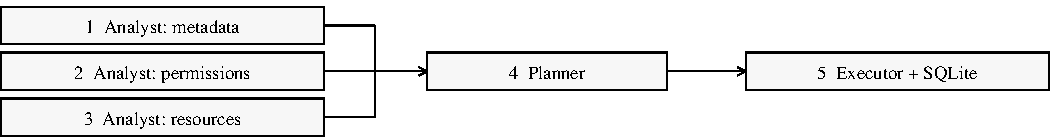
\includegraphics[width=\linewidth]{workflow.pdf}
\end{center}
For example, changing the Analyst's reported size from 4,096 to 4,160 made the Planner produce 130 steps instead of 128 (batch 64, two epochs). The incorrect configuration was saved.

\paragraph{Experimental setup}
Four fixed tasks, each repeated three times, cover clean execution and four faults: incorrect intermediate values (\textbf{ERR}), malicious instructions (\textbf{ADV}), a local tool timeout with no output (\textbf{TMO}), and stale information after a source update (\textbf{STL}). If a run fails before injection, we keep it and record that the injected fault was not reached.

\textbf{BASE} checks output structure and source-version consistency at submission. \textbf{VERIFY\_STOP} also compares Analyst and Planner outputs with current sources and recomputes the arithmetic; it stops at the first error without extra LLM calls. \textbf{FULL\_RESTART} receives the faulty result's identity, conditionally undoes owned writes, and reruns BASE once from current sources. Verification and scoring use separate implementations of the same business rules.

\begin{center}
\small
\setlength{\tabcolsep}{4pt}
\renewcommand{\arraystretch}{1.12}
\begin{tabular}{@{}lrrr@{}}
\toprule
\textbf{Condition} & \textbf{BASE: C / W / S} & \textbf{VERIFY: C / W / S} & \textbf{Restart: C / W / S} \\
\midrule
Clean & 10 / 2 / 0 & 9 / 0 / 3 & - \\
ERR & 0 / 12 / 0 & 0 / 0 / 12 & 10 / 2 / 0 \\
ADV & 12 / 0 / 0 & 10 / 0 / 2 & Not needed (12) \\
TMO & 0 / 0 / 12 & 0 / 0 / 12 & 10 / 2 / 0 \\
STL & 0 / 0 / 12 & 0 / 0 / 12 & 6 / 6 / 0 \\
\bottomrule
\end{tabular}
\end{center}
{\footnotesize Table 1. C: correct completion; W: incorrect configuration written; S: stopped. The 168 scheduled rows include 12 unnecessary ADV restarts; 156 workflows executed. Stops and wrong writes are separate outcomes.\par}

\paragraph{Propagation and verification}
The 12 BASE ERR injections produced \textbf{18 incorrect downstream results and 12 wrong writes}. VERIFY blocked all 11 ERR injections that reached their targets; one run stopped earlier on a natural error. Its three clean-run stops also caught natural model errors, with no false rejection observed. STL produced 12 incorrect descendants, but version checks blocked their writes. Timeouts stopped the workflow before a downstream result existed. All 12 BASE ADV messages were delivered without achieving their attack goals.

\section{Restart costs and the next phase}
\paragraph{A restart can produce a new wrong answer}
\textbf{Full restart was correct in 26 of 36 actual restarts. The other 10 runs wrote incorrect configurations} after new copying or arithmetic errors. The 38/48 final success count includes 12 ADV tasks that needed no restart. Even without an injected fault, BASE made two wrong writes in 12 clean runs.

All 15 investigated clean/restart error cases came from two boundary tasks: 4,097 was copied as 4,096, or 2,049 examples with batch 256 and three epochs produced 24 steps rather than 27. For STL, restarting refreshed the changed sources, but re-generation still produced errors. Of 135 discarded model calls, \textbf{63 outputs still matched current sources at the checkpoint}. They are reuse candidates, not savings already achieved. Phase 2 will test whether retaining checked results also reduces new errors during recovery.

\begin{center}
\small
\setlength{\tabcolsep}{4pt}
\renewcommand{\arraystretch}{1.12}
\begin{tabular}{@{}lrr@{}}
\toprule
\textbf{Method} & \textbf{Executed workflows} & \textbf{Model calls} \\
\midrule
BASE & 60 & 255 \\
VERIFY\_STOP & 60 & 167 \\
FULL\_RESTART & 36 & 180 \\
Total & 156 & 602 \\
\bottomrule
\end{tabular}
\end{center}
{\footnotesize Table 2. The main experiment cost about 3.24 US cents at the recorded token prices. VERIFY used fewer calls because it often stopped early. Across its 60 runs, verification averaged 3.3 extra source reads and 2.7 ms of measured checking time.\par}

A separate permission/resource study produced \textbf{24 unsafe write proposals in each group} (48 runs per group). Without a final authorization check, 13 were committed; with it, all 24 were rejected. Runs that stopped earlier on model errors do not demonstrate protection. With revised prompts, 21/24 normal tasks completed; 23/24 denial, revocation, or resource-limit trials stopped safely and one had an infrastructure failure. Reuse and re-execution both need current permission checks. Details are in the safety supplement.

\paragraph{Selective recovery: design and an initial result}
Our extension uses the Bank Marketing dataset (41,188 records). An \textbf{Analyst} reads data facts, a \textbf{Planner} chooses a feature bundle and a logistic-regression or random-forest recipe, and a \textbf{Reviewer} accepts training results or requests one adjustment. Deterministic tools train and predict with sklearn on CPU and save a report. The runtime records the messages and file versions each result used.

We compare full restart, conservative dependency-based recovery, and \textbf{early cutoff}, adapted from Skyframe's change pruning [3]. Cutoff reruns a decision and compares its full training specification, including data and code versions. In this pilot, we corrupted the Analyst's row-count summary without changing the data. After correction, both initial and feedback-adjusted specifications matched their originals. CUTOFF reused three artifacts after hash and numerical checks; their other sources and permissions also had to remain valid.

\begin{center}
\small
\setlength{\tabcolsep}{4pt}
\renewcommand{\arraystretch}{1.12}
\begin{tabular}{@{}lrrrrrrr@{}}
\toprule
\textbf{Method} & \textbf{New fits} & \textbf{Reused} & \textbf{\shortstack{Train\\CPU s}} & \textbf{\shortstack{Check\\CPU s}} & \textbf{\shortstack{Total\\CPU s}} & \textbf{\shortstack{Recovery\\wall s}} & \textbf{\shortstack{API cost\\US cents}} \\
\midrule
FULL & 3 & 0 & 15.29 & 13.28 & 28.57 & 48.5 & 0.1082 \\
CONSERVATIVE & 3 & 0 & 15.92 & 13.27 & 29.19 & 47.7 & 0.1078 \\
CUTOFF & 0 & 3 & 0.00 & 13.28 & 13.28 & 29.0 & 0.1166 \\
\bottomrule
\end{tabular}
\end{center}
{\footnotesize Table 3. One checkpoint, one run per method (n=1); final model and metrics matched, with eight model calls each. All methods paid about 13.3 CPU s for artifact checks. CUTOFF avoided FULL's 15.3 CPU s of training and reduced recovery wall time, but its usage-based API cost was 7.7\% higher. Worker times include startup and processing.\par}

The next evaluation covers \textbf{three scenarios with six repetitions each}: changed decisions, row-count errors, and updated data. Methods share a saved state before Reviewer feedback; this pilot followed an approved adjustment. Failed slots remain counted. Source-update recovery is unfinished and included in this plan. We will measure correctness, invalid reuse, duplicate effects, recomputation, latency, and cost. Paired clean runs and a heavier CPU workload will test tracking overhead and break-even fault rates. Four baseline tasks and one pilot do not establish general reliability.

{\footnotesize [1] Li et al., \href{https://arxiv.org/abs/2511.00628}{AgentGit, arXiv:2511.00628}. [2] Yang et al., \href{https://arxiv.org/abs/2605.23311}{DART, arXiv:2605.23311}. [3] Bazel, \href{https://bazel.build/reference/skyframe}{bazel.build/reference/skyframe}.\par}

\clearpage
\appendix
\section{Milestones, tasks, and timing}
\begingroup
\normalsize
\setlength{\parskip}{3pt}
\paragraph{Milestones and deliverables}
\begin{center}
\footnotesize
\setlength{\tabcolsep}{3pt}
\renewcommand{\arraystretch}{1.10}
\begin{tabular}{@{}>{\raggedright\arraybackslash}p{.12\linewidth}>{\raggedright\arraybackslash}p{.19\linewidth}>{\raggedright\arraybackslash}p{.51\linewidth}>{\raggedright\arraybackslash}p{.12\linewidth}@{}}
\toprule
\textbf{Period} & \textbf{Work} & \textbf{Deliverable / completion criterion} & \textbf{Status} \\
\midrule
Oct 20-23 & Baseline and faults & 168 scheduled trials; restart/verification results & Completed \\
Oct 29-31 & Bank pilot & One checked checkpoint; three methods (Table 3) & Completed \\
Nov 2-3 & Phase 1 materials & Report, source, data, logs, and reproduction commands & Completed \\
Nov 2-13 & Recovery experiments & 18 shared states; 54 recovery runs; six clean runs & Planned \\
Nov 2-13 & Runtime failure tests & Zero duplicate actions or overwritten external updates & Planned \\
Nov 14-24 & Overhead and cost & Paired tracking measurements, one heavier workload, rule/verification controls, and break-even curves & Planned \\
Nov 25-Dec 10 & Final analysis & Result tables, variability, limitations, and final artifacts & Planned \\
\bottomrule
\end{tabular}
\end{center}

\paragraph{Recovery experiments (planned)}
Each scenario has six repetitions. The three methods share the same saved failure state, checks, and resource limits.

\textbf{N: Unchanged decision.} Add one to the Analyst's row count. Test whether training can be reused when the corrected plan is unchanged.

\textbf{D: Changed decision.} Replace the Planner's choice with a permitted five-feature logistic-regression recipe. Test whether changed plans force retraining. Correct outputs must match the corrected plan and current data.

\textbf{U: Updated data.} Apply N and change one training value. Test whether new data invalidates an old model even when the recipe is unchanged.

Metrics include correct completion, invalid reuse, duplicate actions, recomputation, latency, fees, and plan changes. Model-consistency checks are described in the workflow guide.

\paragraph{Runtime tests and interruptions (planned)}
Fake-tool tests will interrupt a completed action before its receipt is saved, repeat a Reviewer approval, and introduce a concurrent data update. Recovery must look up actions by ID, avoid duplicate effects, and preserve others' updates.

429/502 or missing token-usage data stops the batch. Interrupted runs remain infrastructure failures; once service and accounting checks pass, only unstarted runs continue in a new batch. Unknown effects stay unresolved. We will report negative savings and completion rates alongside costs.

\small
\paragraph{Configuration tasks}
\begin{center}
\footnotesize
\setlength{\tabcolsep}{4pt}
\renewcommand{\arraystretch}{1.12}
\begin{tabular}{@{}lrrrr@{}}
\toprule
\textbf{Task} & \textbf{Examples} & \textbf{Batch / epochs} & \textbf{Requested / cap} & \textbf{Correct steps / workers} \\
\midrule
eval01 & 4,096 & 64 / 2 & 2 / 8 & 128 / 2 \\
eval02 & 4,097 & 64 / 2 & 8 / 3 & 130 / 3 \\
eval03 & 17 & 128 / 3 & 1 / 4 & 3 / 1 \\
eval08 & 2,049 & 256 / 3 & 5 / 2 & 27 / 2 \\
\bottomrule
\end{tabular}
\end{center}
All 602 baseline requests used TritonAI api-glm-5.3-flash, low reasoning effort, and a 768-token output limit. Temperature and seed were not set. The Bank pilot used temperature 0 and training seed 17, with Python 3.10.12, sklearn 1.3.0, one CPU thread, and an 8 GiB limit. Pilot final AP was 0.2306 and ROC-AUC 0.6733. On this imbalanced task, F1 at the fixed 0.5 threshold was zero; no threshold tuning was performed.

\paragraph{Recorded execution times}
\begin{center}
\footnotesize
\setlength{\tabcolsep}{4pt}
\renewcommand{\arraystretch}{1.12}
\begin{tabular}{@{}lrrrr@{}}
\toprule
\textbf{Condition} & \textbf{BASE} & \textbf{VERIFY} & \textbf{Restart only} & \textbf{Initial + restart} \\
\midrule
Clean & 4.96 [4.64, 12.80] & 4.75 [0.67, 5.00] & - & - \\
ERR & 4.88 [4.68, 5.41] & 0.91 [0.68, 3.91] & 5.06 [4.76, 5.39] & 9.96 [9.64, 10.47] \\
TMO & 2.21 [1.10, 3.57] & 1.73 [0.70, 2.88] & 5.89 [5.69, 7.30] & 8.33 [6.80, 9.60] \\
STL & 4.83 [4.61, 5.21] & 1.75 [0.61, 2.76] & 5.07 [4.80, 5.40] & 9.88 [9.63, 10.20] \\
\bottomrule
\end{tabular}
\end{center}
{\footnotesize Table A1. Seconds: median [minimum, maximum], 12 runs per populated cell. Initial + restart is calculated per pair before aggregation. These recorded windows omit handoff, audit, and export gaps; shorter stopped runs are not faster successful executions. Ten VERIFY TMO rows timed out; two stopped before the timeout on a natural error.\par}

\endgroup
\end{document}
